\section*{Performance Measurement Results}

The purpose of this section is to evaluate and compare the performance of the four different hardware configurations. This assessment will help us determine the most suitable configuration for achieving the desired balance between processing power, accuracy, and energy efficiency.\\


\textbf{Detection accuracy (precision, recall, F1-score)}
\begin{itemize}

\item Precision: Precision is a measure of how many of the detected objects are actually relevant. It is calculated as the number of true positives (TP) divided by the sum of true positives and false positives (FP). A high precision indicates that the object detection system is good at identifying relevant objects while avoiding false detections. 
Precision = TP / (TP + FP)

\item Recall: Recall is a measure of how many of the relevant objects are detected by the system. It is calculated as the number of true positives (TP) divided by the sum of true positives and false negatives (FN). A high recall indicates that the object detection system is good at finding all the relevant objects in the scene.
Recall = TP / (TP + FN)

\item F1-score: The F1-score is the harmonic mean of precision and recall, providing a single metric that balances both precision and recall. This is useful when you want to compare the performance of different object detection systems, especially when there's a trade-off between precision and recall. An F1-score closer to 1 indicates a better-performing object detection system.
F1-score = 2 * (Precision * Recall) / (Precision + Recall) \cite{preandrec}[p. 155-156]\\ 
\end{itemize}
\newpage
\textbf{Frame Rate}
\begin{itemize}
\item Frame Rate, often measured in frames per second (fps), refers to the speed at which the system can process consecutive images for object detection. It represents the number of images the system can analyze and generate object detection results for within a second.
\item Higher frame rates indicate better performance, as the system can analyze more images in a given period. This is particularly important for drone applications, where real-time or near-real-time object detection is crucial for seamless operation and rapid decision-making.\\
\end{itemize}

\textbf{Power consumption}
\begin{itemize}
 \item Power consumption refers to the amount of electrical power used by the edge configurations while performing object detection tasks. It is measured in watts (W) and is obtained by monitoring the current and voltage supplied to the device during operation.
\item Lower power consumption is generally more desirable, as it indicates higher energy efficiency and can result in longer flight times for the drone. Comparing the power consumption of the four configurations can help determine which option is better suited for a lightweight drone, where battery life and weight are critical factors.\\
\end{itemize}

\textbf{Weight Efficiency}
\begin{itemize}
    \item Weight efficiency refers to the total weight of the configuration, including the computational hardware (like the Jetson Nano or Raspberry Pi), any attached accelerators (like the Google Coral TPU), and necessary components for their function (like heat sinks, cables, power supply, etc.). In the context of drones, lower weight is preferable as it can lead to longer flight times and improved maneuverability. \\
\end{itemize}

\textbf{Complexity (Ease of Setup and Operation)}
\begin{itemize}
\item Complexity in this context refers to the level of difficulty involved in setting up and operating the object detection system. This includes tasks such as installing and configuring the necessary software, implementing the object detection model, troubleshooting issues, and managing the system during operation.
\item 1 represents a very complex system that is difficult to set up and operate. This might include challenges such as complicated installation procedures, hard-to-resolve errors, poor documentation, a steep learning curve, and significant maintenance requirements.
\item 10 represents an easy-to-use system that is straightforward to set up and operate. This might include factors such as clear and thorough documentation, simple installation procedures, easy-to-use tools and interfaces, minimal troubleshooting requirements, and low maintenance needs.\\
\end{itemize}

\textbf{Results}
\begin{table}[ht]
\centering
\begin{tabular}
{ |c|c|c|c|c|c|c|c| } 
\hline
Configuration & config 1 & config 1 & config 2 & config 2 & config 3 & config 3 & config 4\\
              & yolov5n & yolov5s  &  edl0    &  edl1     & edl0    & edl1     & blob\\
\hline
Precision & 0.991 & 0.995 & 0.945 & 0.924 & 0.945 &  0.924 & 0.96\\
\hline
Recall & 1.00 & 1.00 & 0.516 & 0.580 & 0.516 & 0.580 & 0.25\\
\hline
F1-score & 0.96 & 0.96 & 0.667 & 0.712 & 0.667 & 0.712 & 0.399\\
\hline
Avg FPS over 30 sec & 11.03 & 5.966 & 24.64 & 16.46 & 5.70 & 3.92 & 23.33\\
\hline
Power Consumption (W) & 10.8 &  & 11.7 & & 11.7 & & 7,2 W \\
\hline
Weight (g) & 246.1 &  & 87.6 & & 43.3 & & 51.1 \\
\hline
Complexity & 2 &  & 9 & & 9 & & 7 \\
\hline
Price & 124\$ &  & 145\$ & & 100\$ & & 85\$ \\
\hline
\end{tabular}
\caption{Results}
\label{tab:målinger}
\end{table}

\newpage


\begin{figure}[h]
    \centering
    \begin{subfigure}{0.45\textwidth}
        \centering
        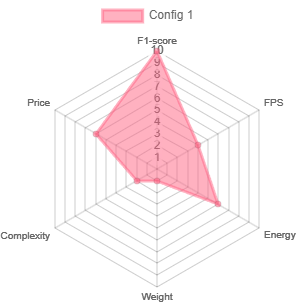
\includegraphics[width=\linewidth]{evenbilder/spiderdiag/config1.png}
        \caption{Config 1 results}
        \label{fig:a}
    \end{subfigure}
    \hfill
    \begin{subfigure}{0.45\textwidth}
        \centering
        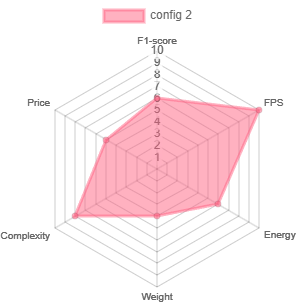
\includegraphics[width=\linewidth]{evenbilder/spiderdiag/config2.png}
        \caption{Config 2 results}
        \label{fig:b}
    \end{subfigure}
    \\ % this line break will put the next two images on the next line
    \begin{subfigure}{0.45\textwidth}
        \centering
        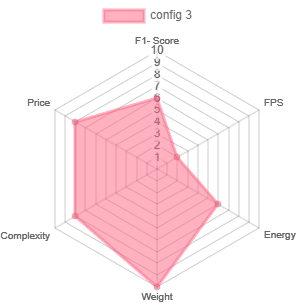
\includegraphics[width=\linewidth]{evenbilder/spiderdiag/config3.png}
        \caption{Config 3 results}
        \label{fig:c}
    \end{subfigure}
    \hfill
    \begin{subfigure}{0.45\textwidth}
        \centering
        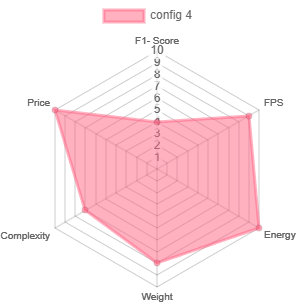
\includegraphics[width=\linewidth]{evenbilder/spiderdiag/config4.png}
        \caption{Config 4 results}
        \label{fig:d}
    \end{subfigure}
    \caption{Results represented in spider diagrams}
    \label{fig:fourgrid}
\end{figure}

\newpage

\section{Config1}

The following figure show the FPS performance of configuration 1 while running object detection.
We ended up testing two Yolo models, nano and small. 
\begin{figure}[H]
    \centering
    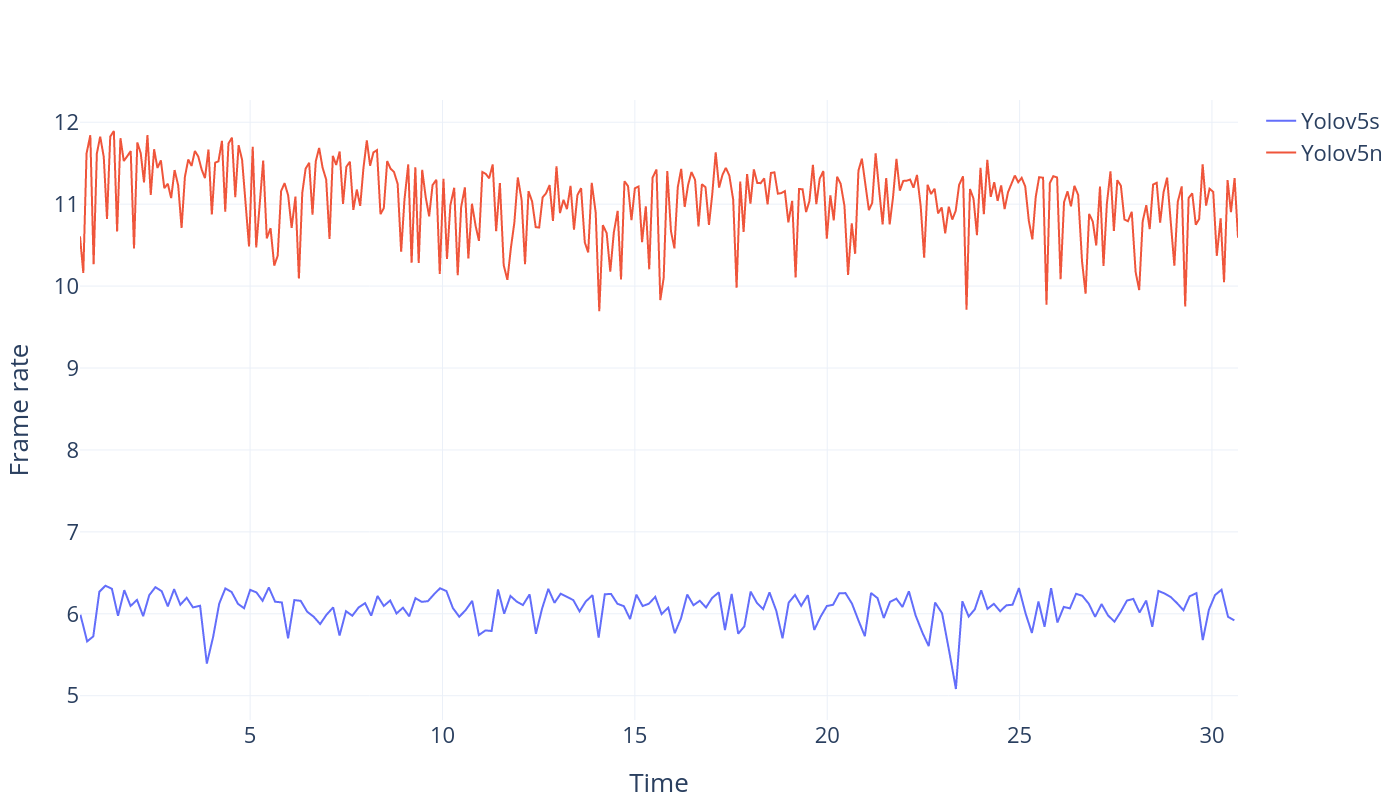
\includegraphics[width=\textwidth]{evenbilder/Framerate yolo.png}
    \caption{Yolov5 nano versus small model FPS}
    \label{fig:yolofps}
\end{figure}


\section{Config2 \& Config3}

Both the EfficientDet Lite 0 and EfficientDet Lite 1 models has been benchmarked on the following three hardware configurations:
\begin{itemize}
    \item Raspberry Pi 4B       w/ Coral USB Accelerator (Config 2)
    \item Raspberry Pi Zero2    w/ Coral USB Accelerator (Config 3)
    \item Raspberry Pi 3B+      w/ Coral USB Accelerator
\end{itemize}

All three hardware configurations has been benchmarked by running the Docker-container at "benchmark/coral-1xRPi" from the "Aerial-Edge/Drone" repository \cite{github-Aerial-Edge_Drone} with the latest Raspberry Pi OS Lite (64-bit) natively installed on a Class A2 SDXC-card.

\subsection{EfficientDet Lite 0}
\begin{figure}[H]
    \centering
    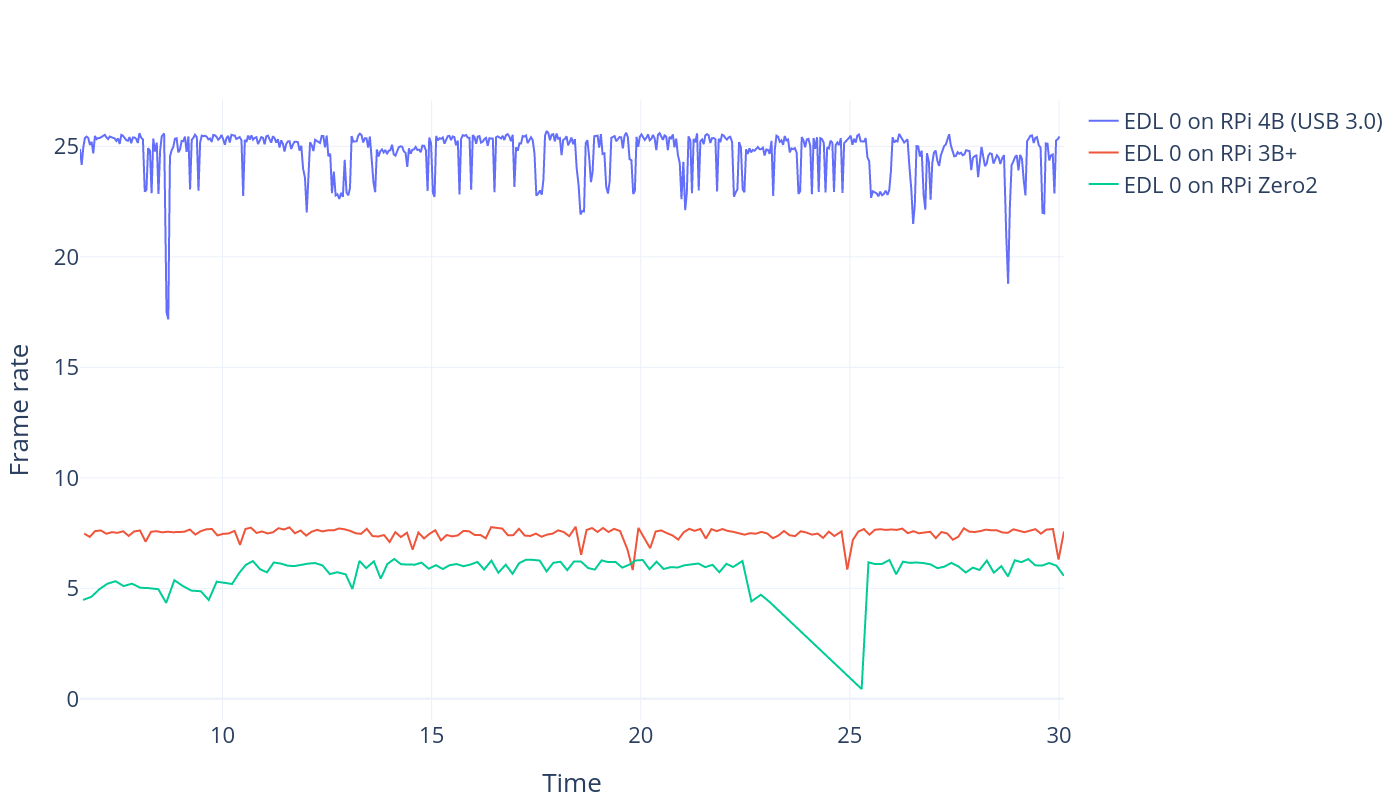
\includegraphics[width=\textwidth]{fig/plots/EDL0.png}
    \caption{EfficientDet Lite 0 on various Raspberry Pies}
    \label{fig:edl0}
\end{figure}

\newpage

\subsection{EfficientDet Lite 1}
\begin{figure}[H]
    \centering
    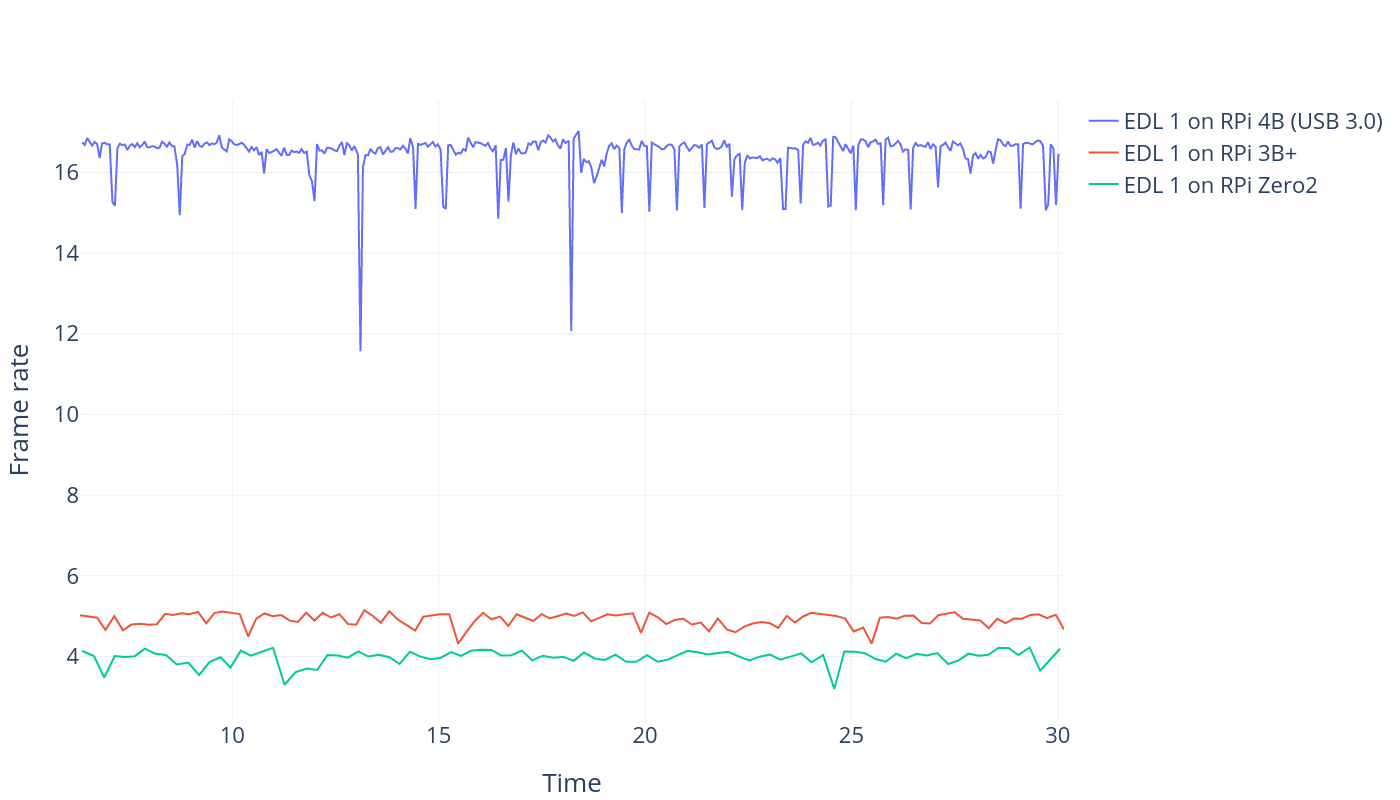
\includegraphics[width=\textwidth]{fig/plots/EDL1.png}
    \caption{EfficientDet Lite 1 on various Raspberry Pies}
    \label{fig:edl1}
\end{figure}

\newpage

\begin{figure}[H]
    \centering
    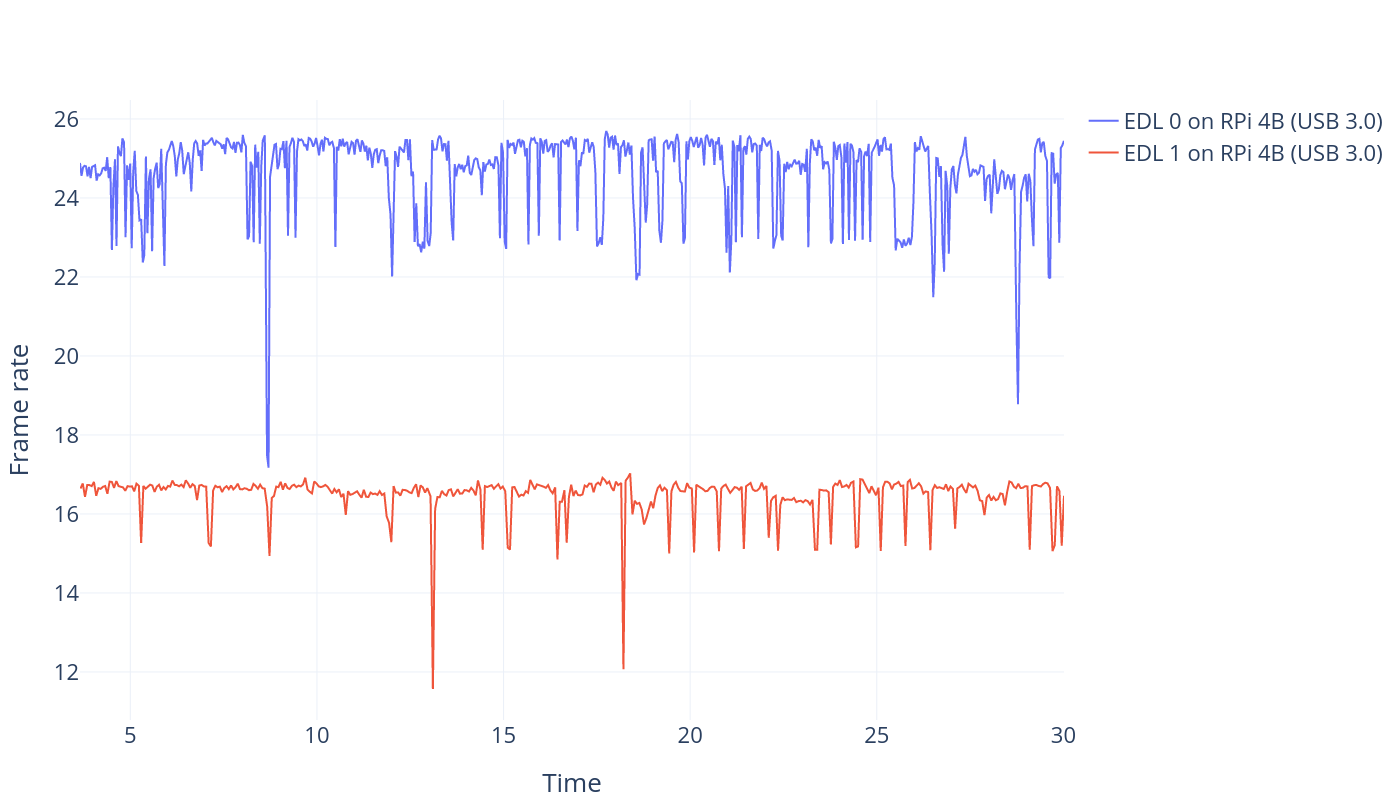
\includegraphics[width=\textwidth]{fig/plots/EDL0_vs_EDL1.png}
    \caption{EfficientDet Lite 0 compared to EfficientDet Lite 1 on Raspberry Pi 4B}
    \label{fig:edl0_vs_edl1}
\end{figure}

\newpage

\subsection{USB 3.0 vs. USB 2.0}

Plugging the Coral USB Accelerator to a USB 2.0-port instead of 3.0-port pretty much halves the frame rate during the object-detection benchmark. This is consistent with the Coral's tech specs\cite{CoralTPU} which claims that the USB Accelerator is compatible with USB 2.0 but the inferencing speed is slower. Note that both the Raspberry Pi 3B+ and Zero 2 only have USB 2.0 ports but the 4B still produces a substantially higher frame rate than these two when it also is connected on USB 2.0.

\begin{figure}[H]
    \centering
    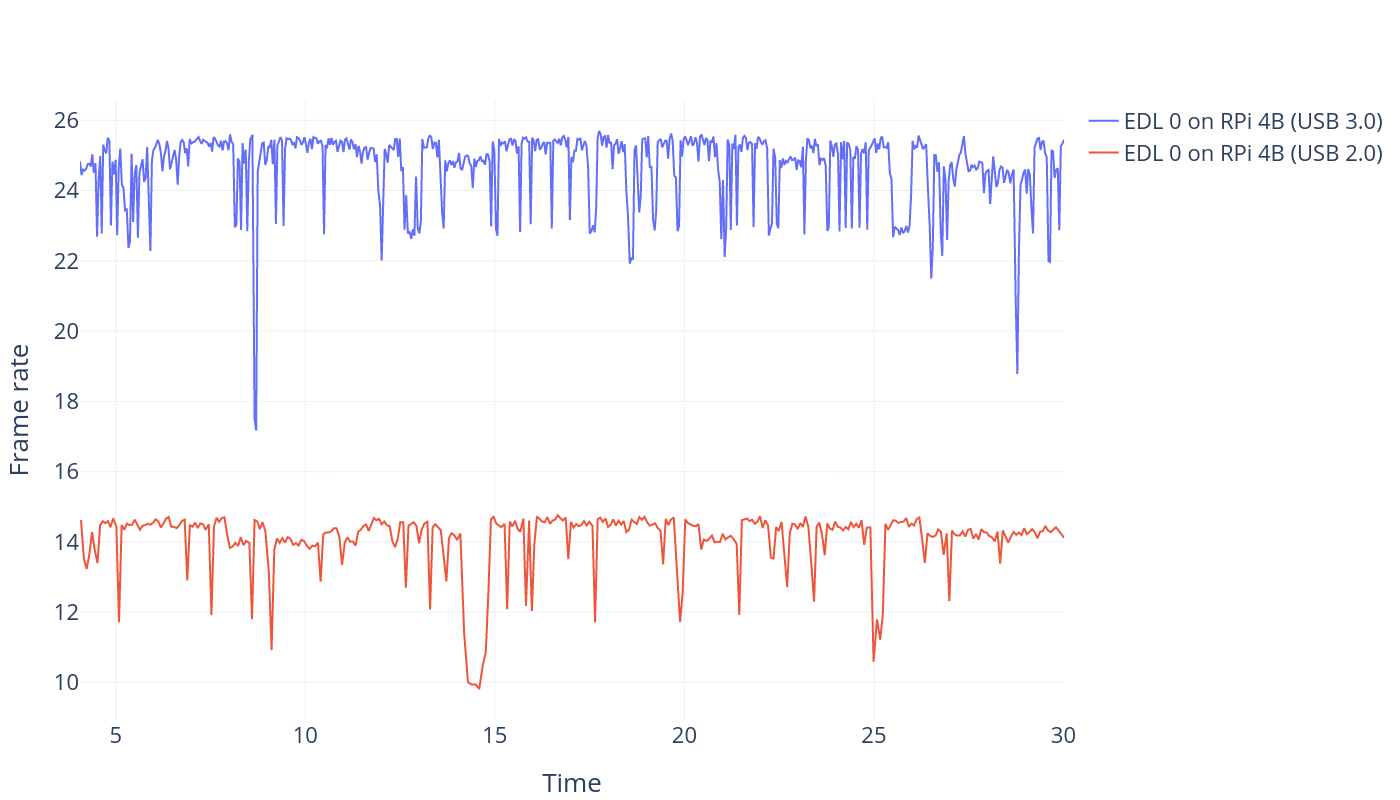
\includegraphics[width=\textwidth]{fig/plots/EDL0-USB_3_vs_2.png}
    \caption{EfficientDet Lite 0, USB 3.0 vs 2.0 on RPi 4B}
    \label{fig:edl0-usb_2_vs_3}
\end{figure}

\begin{figure}[H]
    \centering
    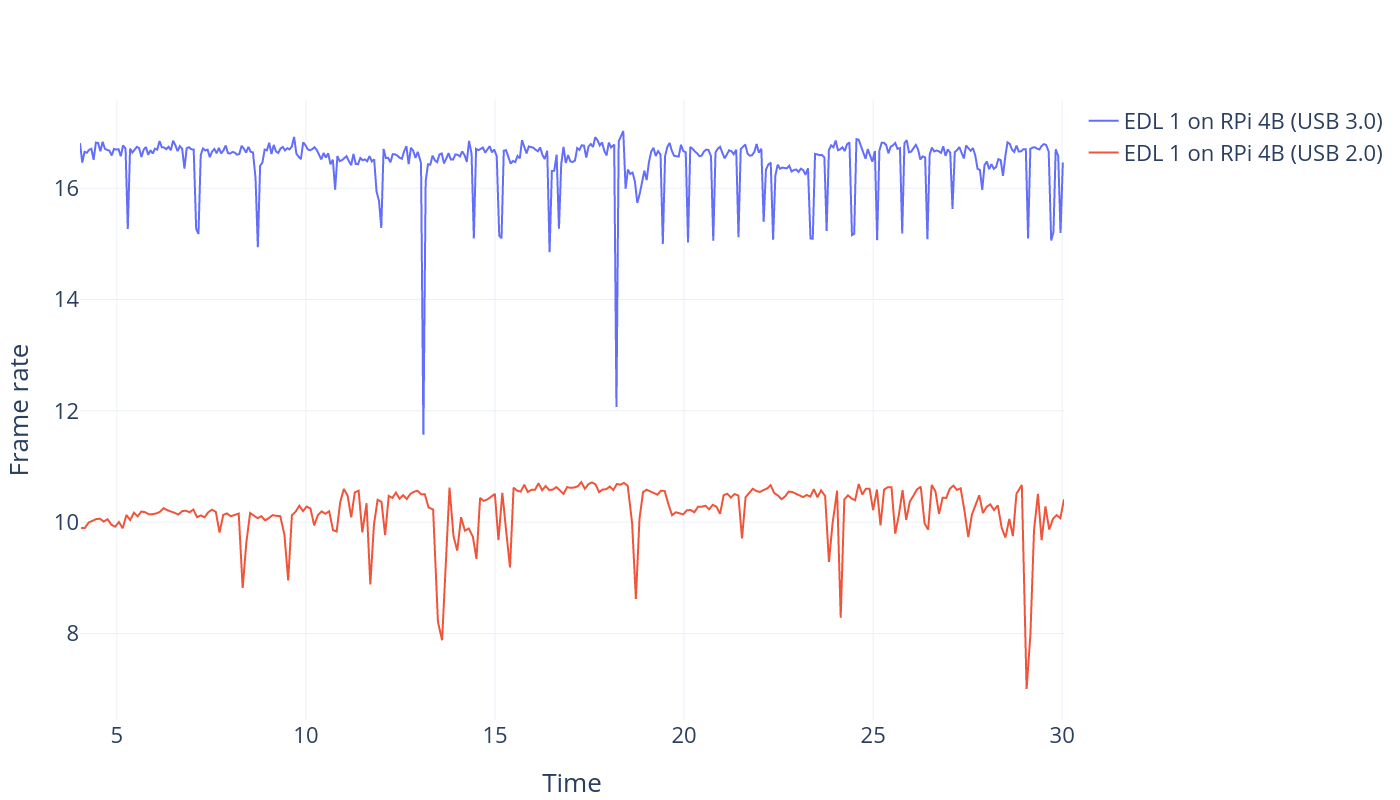
\includegraphics[width=\textwidth]{fig/plots/EDL1-USB_3_vs_2.png}
    \caption{EfficientDet Lite 1, USB 3.0 vs 2.0 on RPi 4B}
    \label{fig:edl1-usb_2_vs_3}
\end{figure}

\newpage

\section{Config4}

The following figure displays the frame per second (FPS) performance of Configuration 4 while tracking a single object over a 30-second interval with our final blob detection: \ref{ros2nodeC4}

\begin{figure}[h]
    \centering
    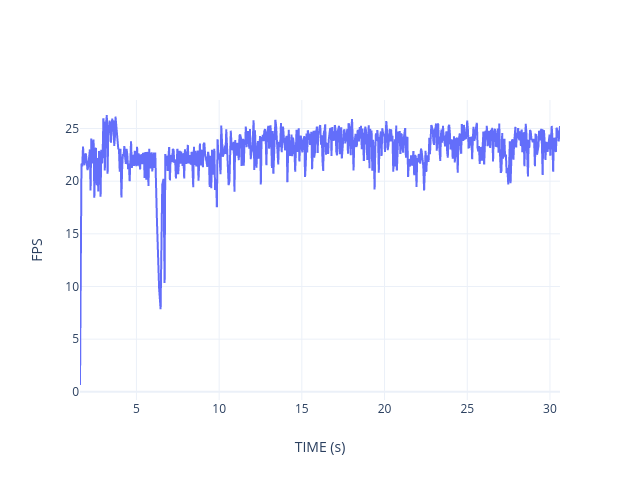
\includegraphics[width=\textwidth]{sindrebilder/config4_fps.png}
    \caption{FPS, Configuration 4}
    \label{fig:fpsConfig4}
\end{figure}

